\documentclass[aspectratio=169,11pt]{beamer}
\usepackage[T1]{fontenc}
\usepackage{lmodern}
\usepackage{amsmath,amssymb,graphicx,tikz}
\usetikzlibrary{arrows.meta,positioning}
\definecolor{ink}{HTML}{153349}
\definecolor{teal}{HTML}{087F8C}
\definecolor{muted}{HTML}{566675}
\definecolor{pale}{HTML}{EDF5F6}
\definecolor{tiblue}{HTML}{0A4F8C}
\definecolor{carrierred}{HTML}{B3361F}
\setbeamercolor{normal text}{fg=ink,bg=white}
\setbeamercolor{structure}{fg=teal}
\setbeamercolor{frametitle}{fg=ink}
\setbeamerfont{frametitle}{size=\large,series=\bfseries}
\setbeamertemplate{navigation symbols}{}
\setbeamersize{text margin left=8mm,text margin right=8mm}
\setbeamertemplate{frametitle}[default][left]
\addtobeamertemplate{frametitle}{\vspace{2mm}}{}
\setbeamertemplate{footline}{%
  \hspace{8mm}\color{muted}\fontsize{6.5}{8}\selectfont
  TI: the cortical column as a tuned receiver\hfill 10 November 2026
  \hspace{5mm}\insertframenumber/6\hspace{8mm}\vspace{3mm}}
\setlength{\parskip}{6pt}
\setlength{\abovedisplayskip}{5pt}
\setlength{\belowdisplayskip}{5pt}
\newcommand{\source}[1]{\vfill{\color{muted}\fontsize{7.2}{9}\selectfont #1\par}}
\title{Temporal interference: main results}
\author{G. Ruffini, R. Salvador, B. Mercadal, R. de Palma Aristides,
F. Castaldo, N. Grossman, S. Canals, C. Mirasso}
\date{10 November 2026}
\hypersetup{pdftitle={Temporal interference: six-slide overview},
pdfauthor={Giulio Ruffini and colleagues},
pdfsubject={Main findings of TN0484 / WP0185, draft28}}

\begin{document}

\begin{frame}[t]{Temporal interference: a tuned receiver}
{\fontsize{8.5}{10}\selectfont G. Ruffini, R. Salvador, B. Mercadal, R. de Palma Aristides,\\
F. Castaldo, N. Grossman, S. Canals, C. Mirasso}

Two high-frequency fields can drive a slow neural response at their difference
frequency, which is absent from the applied spectrum.

\vspace{2mm}
\centering
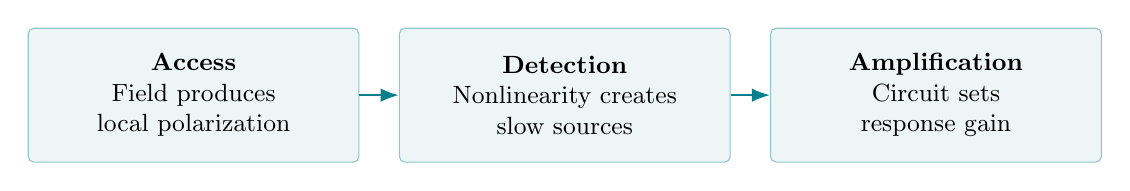
\begin{tikzpicture}[>=Latex,
  stage/.style={draw=teal!45,fill=pale,rounded corners=2pt,
    text width=36mm,minimum height=17mm,align=center,inner sep=3mm,font=\small}]
  \node[stage] (access) {\textbf{Access}\\Field produces\\local polarization};
  \node[stage,right=5mm of access] (detection) {\textbf{Detection}\\Nonlinearity creates\\slow sources};
  \node[stage,right=5mm of detection] (gain) {\textbf{Amplification}\\Circuit sets\\response gain};
  \draw[->,thick,teal] (access) -- (detection);
  \draw[->,thick,teal] (detection) -- (gain);
\end{tikzpicture}
\par\raggedright
For weak quadratic detection, the local carrier polarizations
$\varepsilon_1,\varepsilon_2$ give
\[
\underbrace{\text{beat source}}_{\text{oscillatory}}
\ \propto\ \varepsilon_1\varepsilon_2,
\qquad
\underbrace{\text{steady source}}_{\text{DC-like}}
\ \propto\ \varepsilon_1^2+\varepsilon_2^2.
\]
\source{The stages act in series. Source sign and circuit gain depend on the receiving state.
TN0484 / WP0185, draft28; theoretical mechanisms and one-head spatial illustration.}
\end{frame}

\begin{frame}[t]{The carrier product fixes the quadratic beat map}
\begin{columns}[T,onlytextwidth]
\column{.29\textwidth}
Changing $2+2$ to $1+3$ mA cuts the quadratic beat by 25\%; its spatial pattern stays fixed.

The envelope minimum and mean square move their centroids in opposite directions in this head.

\small These geometric maps do not establish physiological deep selectivity.
\column{.69\textwidth}
\centering
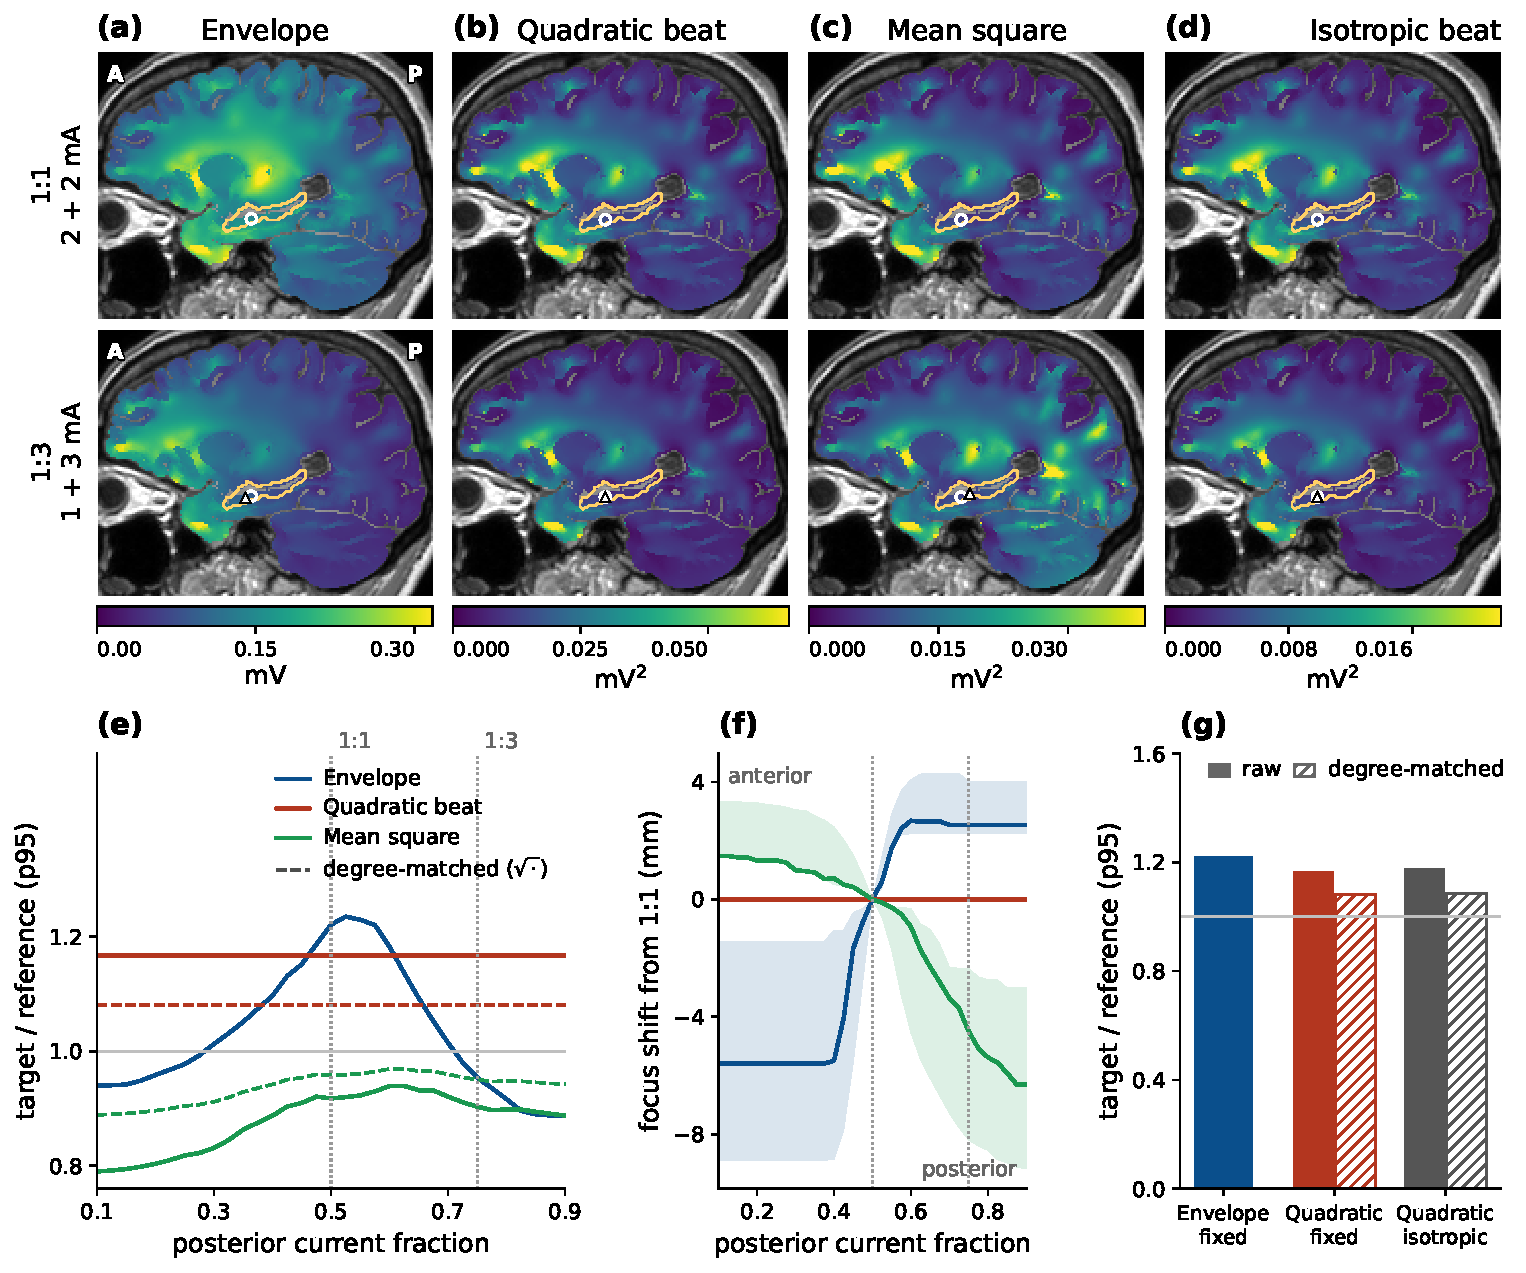
\includegraphics[width=\linewidth,trim=0bp 277bp 181bp 0bp,clip]{figures/fig_fem.pdf}
\end{columns}
\source{Fixed field geometry, polarization directions, and neural state. Centroids use the top 10\% of hippocampal nodes, not global exposure maxima. One IXI002 head, Violante montage. MRI: IXI dataset, CC BY-SA 3.0.}
\end{frame}

\begin{frame}[t]{TI and direct stimulation share the resonant gain}
The detector stays fixed as recurrent coupling increases.
\begin{columns}[T,onlytextwidth]
\column{.48\textwidth}\centering
{\color{teal}\small TI surrogate: gain}\par
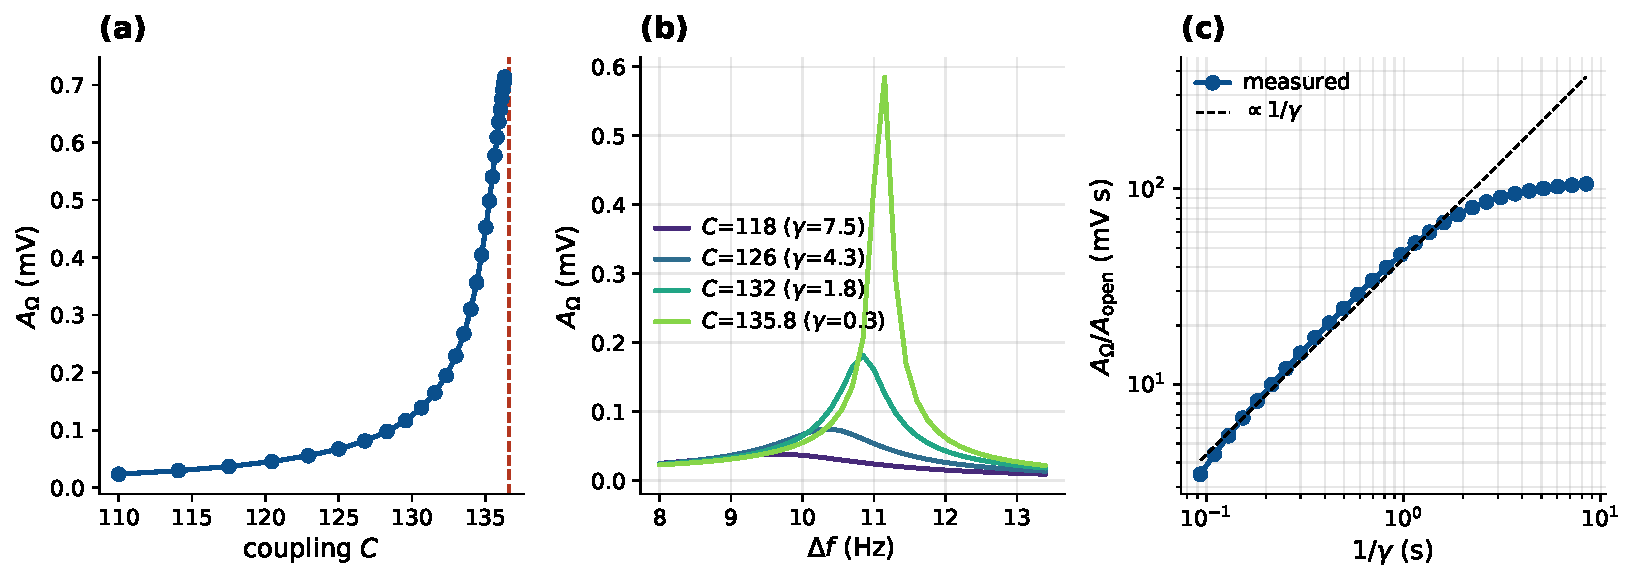
\includegraphics[height=42mm,trim=523bp 0bp 0bp 0bp,clip]{figures/fig_jcurve.pdf}
\column{.48\textwidth}\centering
{\color{teal}\small Direct tACS: response amplitude}\par
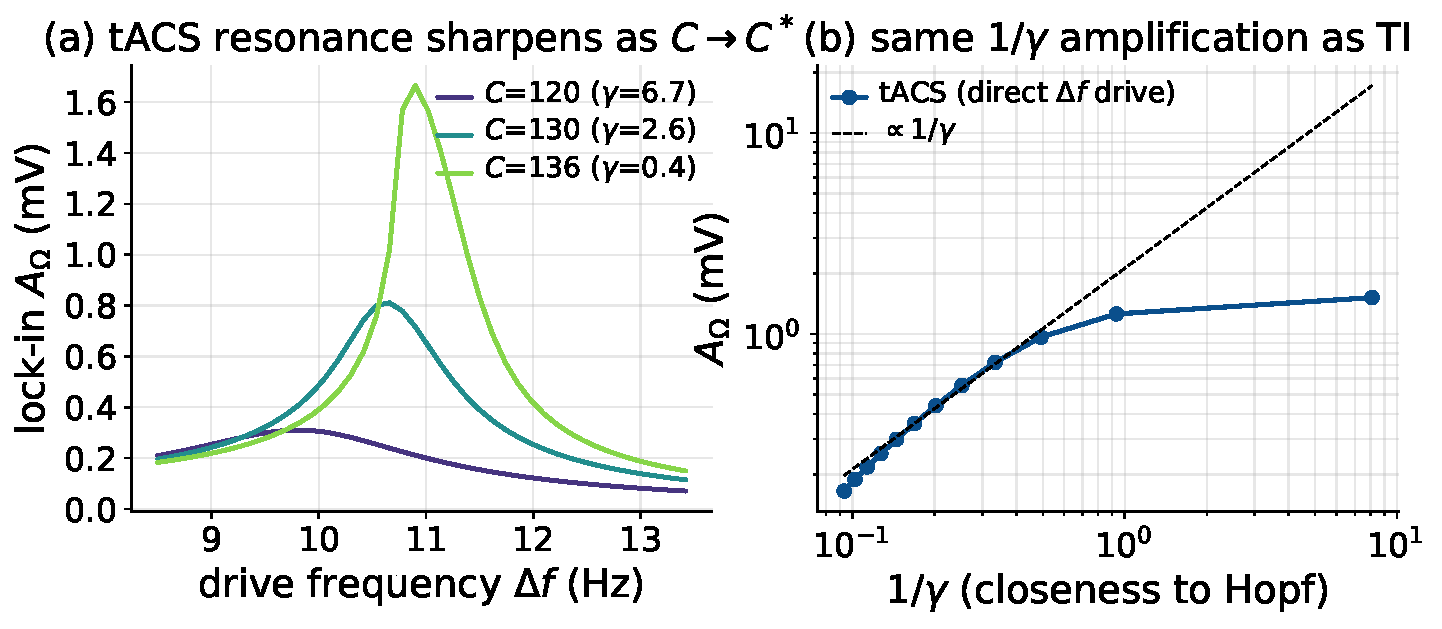
\includegraphics[height=42mm,trim=337bp 0bp 0bp 0bp,clip]{figures/fig_tacs_jcurve.pdf}
\end{columns}
Near instability, gain grows as inverse damping; finite forcing saturates it.
\source{Jansen--Rit model at a fixed operating point. TI uses an amplitude-modulated surrogate here.
tACS: transcranial alternating-current stimulation.
$\gamma$: modal damping; $A_\Omega$: beat-frequency voltage amplitude;
$A_{\rm open}$: local rate-source amplitude. TI and tACS share the linear amplifier at the same state and readout.}
\end{frame}

\begin{frame}[t]{Membrane dynamics can reverse the steady shift}
\begin{columns}[T,onlytextwidth]
\column{.58\textwidth}
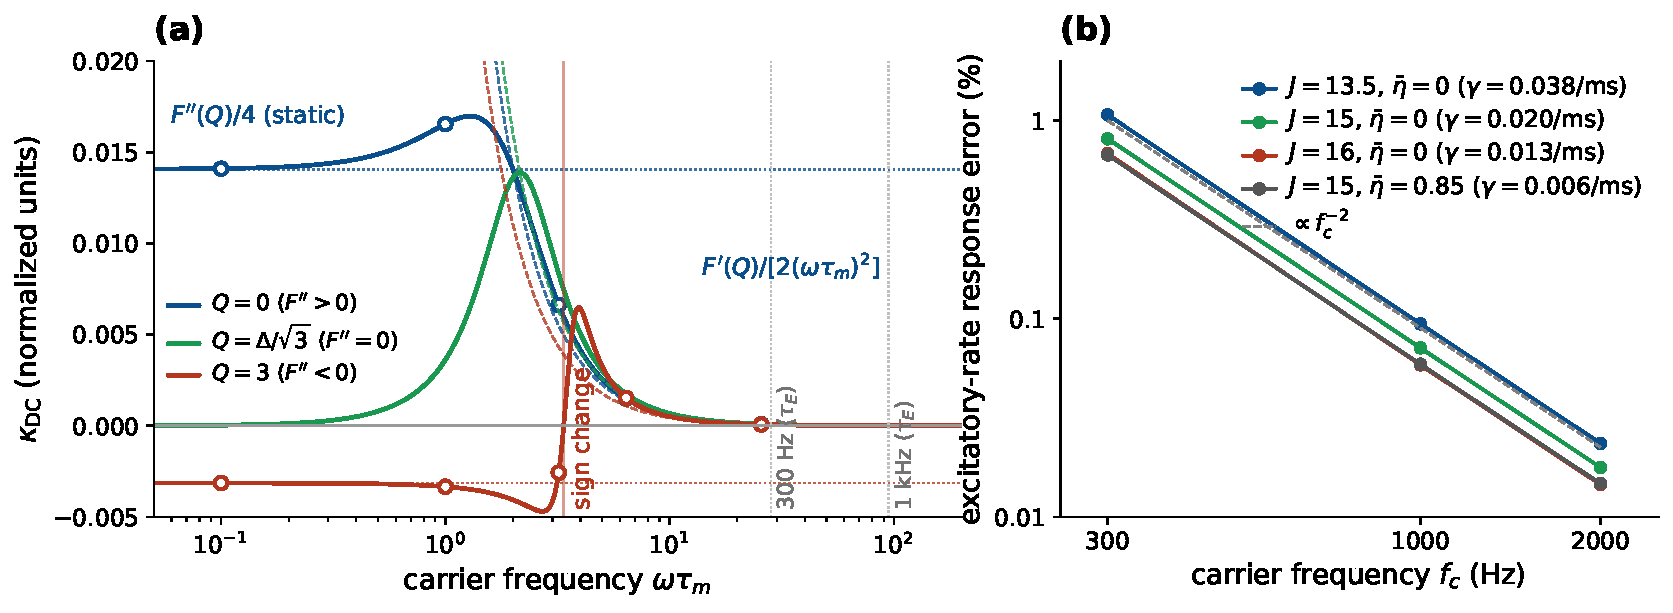
\includegraphics[width=\linewidth,trim=0bp 0bp 354bp 0bp,clip]{figures/fig_mpr_crossover.pdf}
\column{.38\textwidth}
Slow inputs follow the curvature of the static rate curve.

At fast carriers, the quadratic integrate-and-fire model gives a positive steady shift,
even where static curvature predicts a negative one.

The DC-like source's sign depends on local dynamics.
\end{columns}
\source{Weak local rectification at fixed synaptic input.
$\kappa_{\rm DC}$: steady-response coefficient; $F(Q)$: dimensionless steady rate at drive $Q$;
$\omega$: carrier angular frequency; $\tau_m$: membrane time;
$\Delta$: drive-distribution half-width.}
\end{frame}

\begin{frame}[t]{A steady shift can induce gamma without a beat}
At strong input, an unmodulated carrier and TI both induce gamma at matched root-mean-square (RMS) input current.

\begin{columns}[c,onlytextwidth]
\column{.64\textwidth}
\centering
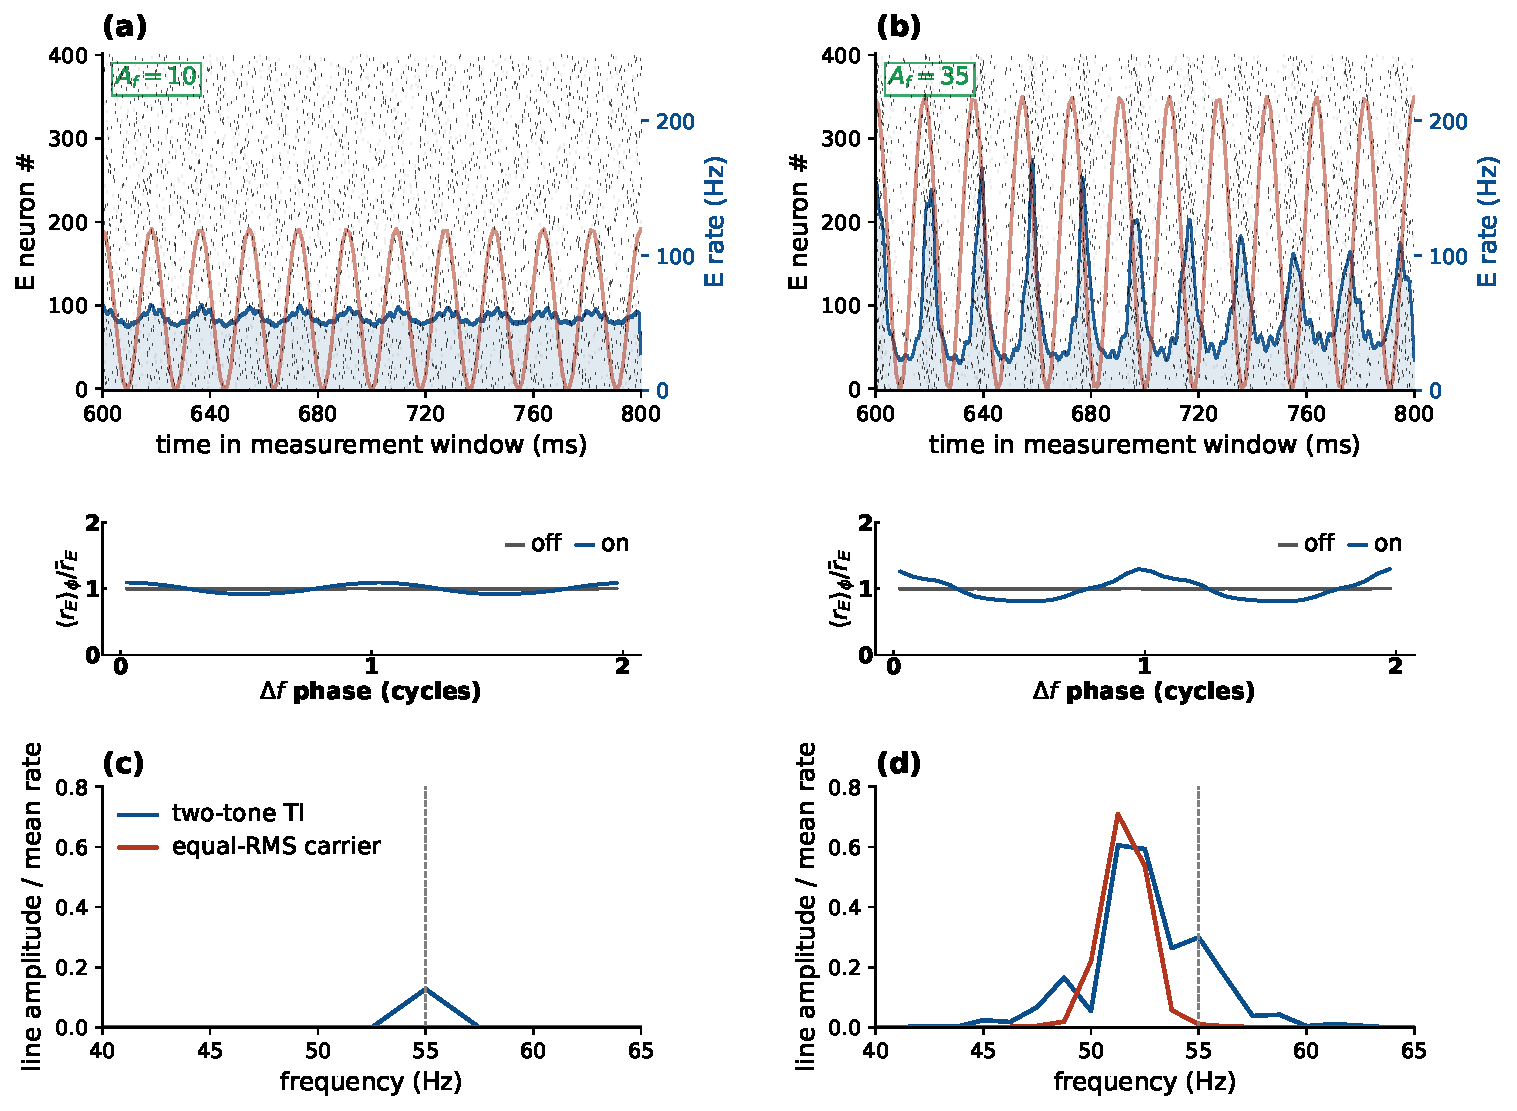
\includegraphics[width=\linewidth,trim=365bp 0bp 0bp 354bp,clip]{figures/fig_qif_regimes.pdf}\par
{\fontsize{9}{11}\selectfont
\tikz[baseline=-.5ex]\draw[tiblue,line width=1pt] (0,0)--(.5,0);\enspace TI\qquad
\tikz[baseline=-.5ex]\draw[carrierred,line width=1pt] (0,0)--(.5,0);\enspace Unmodulated carrier}
\column{.32\textwidth}
Both responses peak near 51 Hz. TI also has a 55 Hz beat.

An equal-RMS carrier control separates steady-shift effects from beat-dependent responses.
\end{columns}
\source{Excitatory--inhibitory mean field of quadratic integrate-and-fire neurons.
Carrier 300 Hz; TI input amplitude 35 per tone, in model units. This is a mean-field control;
induced gamma does not by itself establish entrainment.}
\end{frame}

\begin{frame}[t]{Membrane access sets the source strength}
\begin{columns}[T,onlytextwidth]
\column{.56\textwidth}
At the Jansen--Rit state studied, TI sources are about 2--5\% of matched direct sources
for carrier polarizations of 0.1--0.3 mV.

At a fixed applied field, carrier access sets the local polarizations. Its strength in tissue remains to be calibrated.

\medskip
Measure local carrier polarization and compare beat and steady responses with the equal-RMS carrier control.
\column{.41\textwidth}
\centering
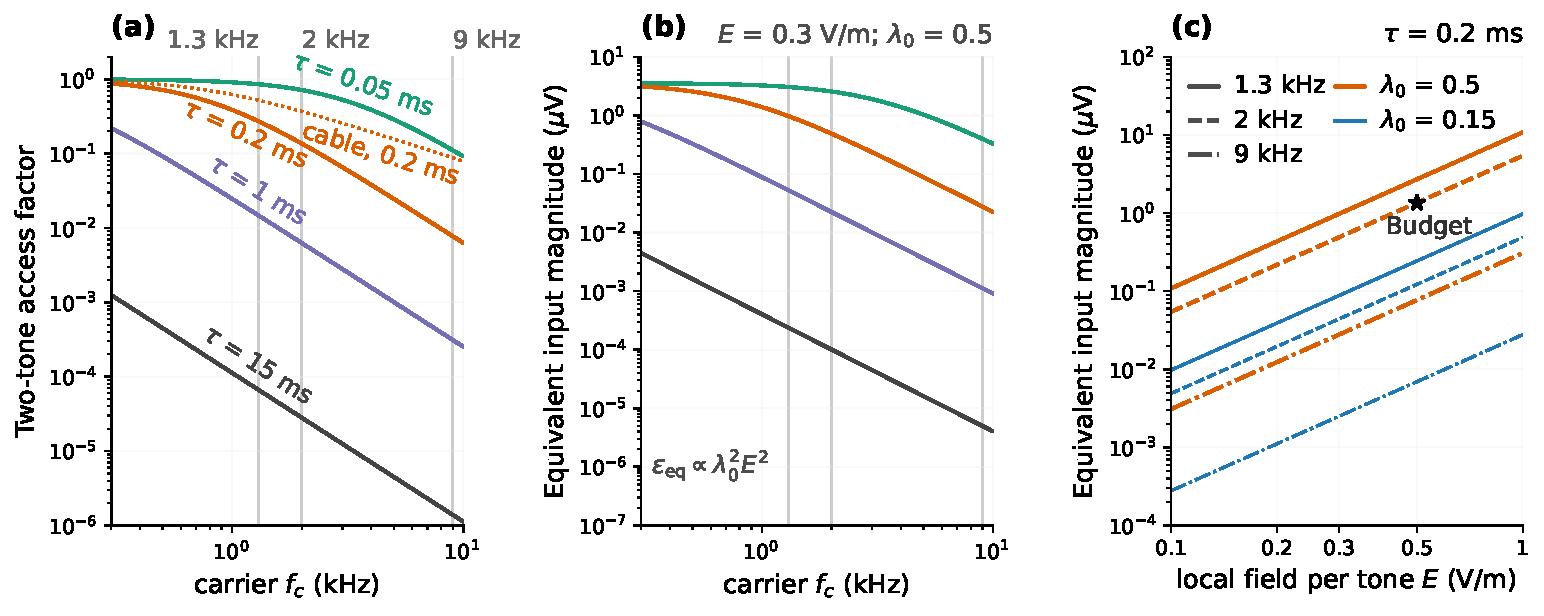
\includegraphics[height=49mm,trim=0bp 0bp 492bp 0bp,clip]{figures/fig_feasibility_khz.pdf}
\end{columns}
\source{Weak-source comparison before circuit gain: each TI carrier and the direct input have the same peak polarization.
Compare steady sources with direct-current stimulation and beat sources with tACS.
Plot: access factor is the product of carrier-transfer magnitudes, which attenuates the quadratic beat at fixed field.
$\tau$: assumed access time. Solid curves: first-order filters; dotted: sealed-cable approximation.}
\end{frame}

\end{document}
